% (The MIT License)
%
% Copyright (c) 2023-2024 Yegor Bugayenko
%
% Permission is hereby granted, free of charge, to any person obtaining a copy
% of this software and associated documentation files (the 'Software'), to deal
% in the Software without restriction, including without limitation the rights
% to use, copy, modify, merge, publish, distribute, sublicense, and/or sell
% copies of the Software, and to permit persons to whom the Software is
% furnished to do so, subject to the following conditions:
%
% The above copyright notice and this permission notice shall be included in all
% copies or substantial portions of the Software.
%
% THE SOFTWARE IS PROVIDED 'AS IS', WITHOUT WARRANTY OF ANY KIND, EXPRESS OR
% IMPLIED, INCLUDING BUT NOT LIMITED TO THE WARRANTIES OF MERCHANTABILITY,
% FITNESS FOR A PARTICULAR PURPOSE AND NONINFRINGEMENT. IN NO EVENT SHALL THE
% AUTHORS OR COPYRIGHT HOLDERS BE LIABLE FOR ANY CLAIM, DAMAGES OR OTHER
% LIABILITY, WHETHER IN AN ACTION OF CONTRACT, TORT OR OTHERWISE, ARISING FROM,
% OUT OF OR IN CONNECTION WITH THE SOFTWARE OR THE USE OR OTHER DEALINGS IN THE
% SOFTWARE.

\documentclass{article}
\usepackage{../osbp}
\newcommand*\thetitle{Reviewing Changes}
\begin{document}

\plush{\osbpTitlePage{4}{TJ83ePwyH_A}}

\qte
  [\nospell{\nospell{Martin Fowler}}]
  {martin-fowler}
  {We should remember that \ul{pre-integration} review grew out of an open-source context where contributions appear impromptu from \ul{weakly connected} developers.}
  {fowler2006}

\thought[bugayenko2015blog0209]{Raise issues, don't resolve them!}

\qte
  [\nospell{Michael Fagan}]
  {michael-fagan}
  {The inspection is not intended to redesign, evaluate alternate design solutions, or to find solutions to errors; it is intended \ul{just} to find errors!}
  {fagan1976design}

\qte
  [\nospell{Frank A. Ackerman}]
  {frank-ackerman}
  {Regardless of the application or the language, you can expect inspections to find from seven to 20 major \ul{defects} per thousand noncomment lines of source code and to find major defects at a \ul{cost} of one to five staff-hours.}
  {ackerman1989software}

\qte
  [\nospell{Mateus Freira dos Santos}]
  {mateus-freira-dos-santos}
  {In software projects with less than 34k lines of code, the number of developers that \ul{never contribute again} after receiving a negative comment on the first pull request is 10.97\%; this number more than doubles to 24.02\% when evaluating projects with more than 197k lines of code.}
  {freira2018analyzing}

\thought{Educate the author}

\qte
  [\nospell{Andrew Sutherland}]
  {andrew-sutherland}
  {The meat of the code review dialog, no matter what the medium, is the \ul{articulation} of design rationale... Engineers find code review dialogs useful for a variety of purposes, but for understanding \ul{design rationale} more than any other.}
  {sutherland2009can}

\qte
  [\nospell{Brendan Cleary}]
  {brendan-cleary}
  {`Raise issues, don't resolve them.' --- this mentality limits a group's ability to \ul{collectively} solve problems and \ul{mentor} developers.}
  {rigby2012contemporary}

\qte
  [\nospell{Alberto Bacchelli}]
  {alberto-bacchelli}
  {Our results show that, although the top motivation driving code reviews is still \ul{finding defects}, the practice and the actual outcomes are \ul{less} about finding errors than expected: Defect related comments comprise a small proportion and mainly cover small logical low-level issues.}
  {bacchelli2013expectations}

\qte
  [\nospell{Peter C. Rigby}]
  {peter-rigby}
  {Contemporary review is performed regularly and quickly just before the code is committed instead of when a larger work product is complete as in inspection. Contemporary reviewers prefers \ul{discussion} and \ul{fixing} code over reporting defects.}
  {rigby2013convergent}

\qte
  [\nospell{Caitlin Sadowski}]
  {caitlin-sadowski}
  {As developers build experience working at Google, the average number of comments on their changes \ul{decreases}... Developers at Google who have started within the past year typically have more than \ul{twice} as many comments per change.}
  {sadowski2018modern}
\pitch{
  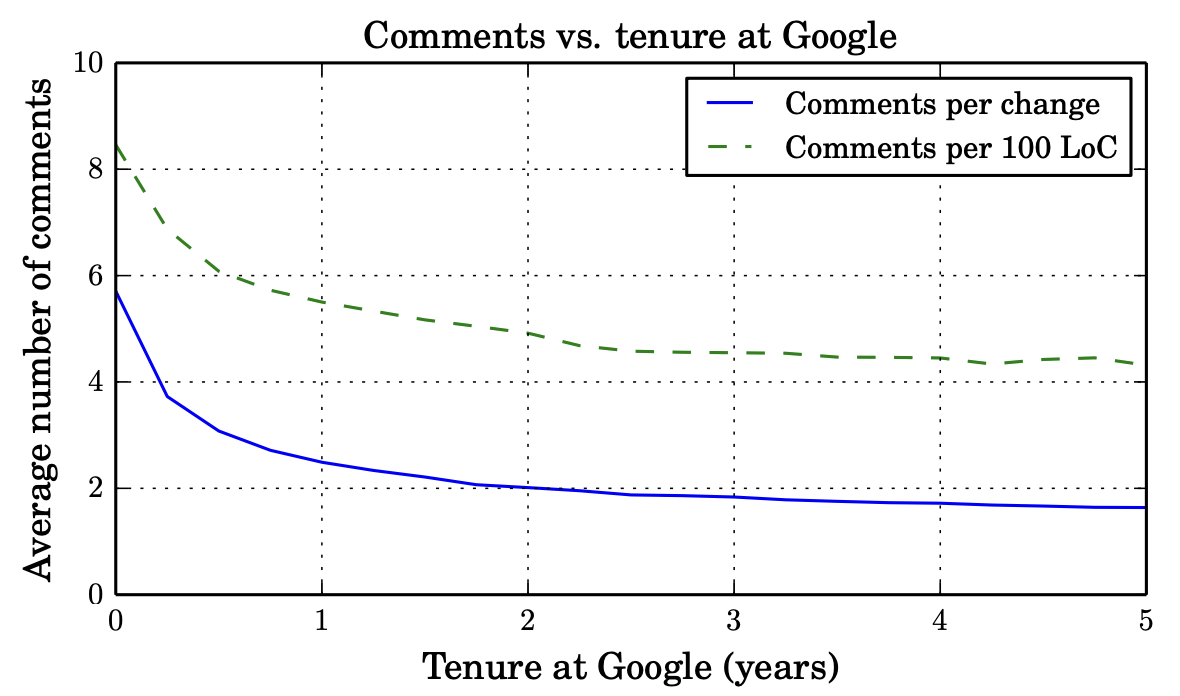
\includegraphics[width=.6\linewidth]{tenure.png}
  \source{sadowski2018modern}}

\thought[bugayenko2019blog1203]{Don't run the code in the branch}

\thought[bugayenko2015blog0622]{Reject it, if it's too big}

\qte
  {eric-raymond}
  {Good programmers know what to write. Great ones know what to \ul{rewrite} (and \ul{reuse}).}
  {raymond1999cathedral}

\qte
  [\nospell{\nospell{Frederic Painchaud}}]
  {frederic-painchaud}
  {To facilitate early and frequent \ul{feedback}, OSS projects tend to review smaller changes than proprietary projects, ranging from 11 to 32 lines in the median case. The small size lets reviewers \ul{focus} on the entire change, and the incrementality reduces reviewers’ preparation time and lets them maintain an overall picture of how the change fits into the system.}
  {rigby2012contemporary}

\pitch{
  \begin{multicols}{2}
  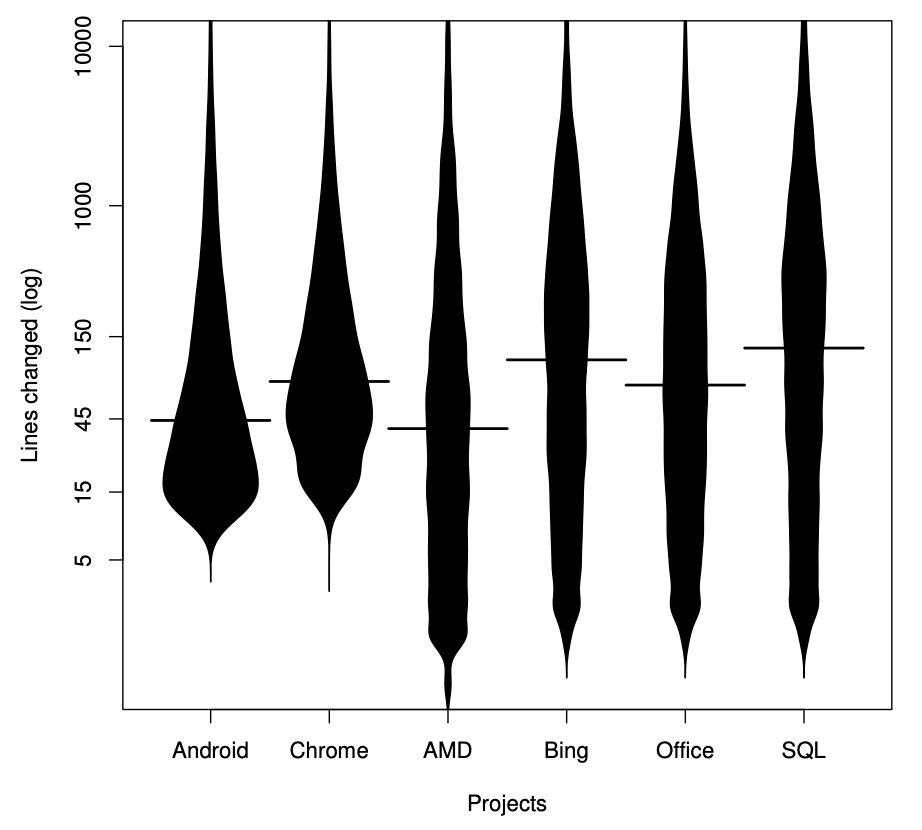
\includegraphics[width=.9\linewidth]{lines-per-pr.png}
  \par\columnbreak\par
  ``Both Android and AMD have a median change size of 44 lines. This median change size is larger than Apache, \ul{25 lines}, and Linux, \ul{32 lines}, but much smaller than Lucent where the number of non-comment lines changed is \ul{263 lines}. Bing, Chrome’s median change is \ul{78 lines} and includes 5 files.''
  \source{rigby2013convergent}
  \end{multicols}}
\pitch{
  \begin{multicols}{2}
  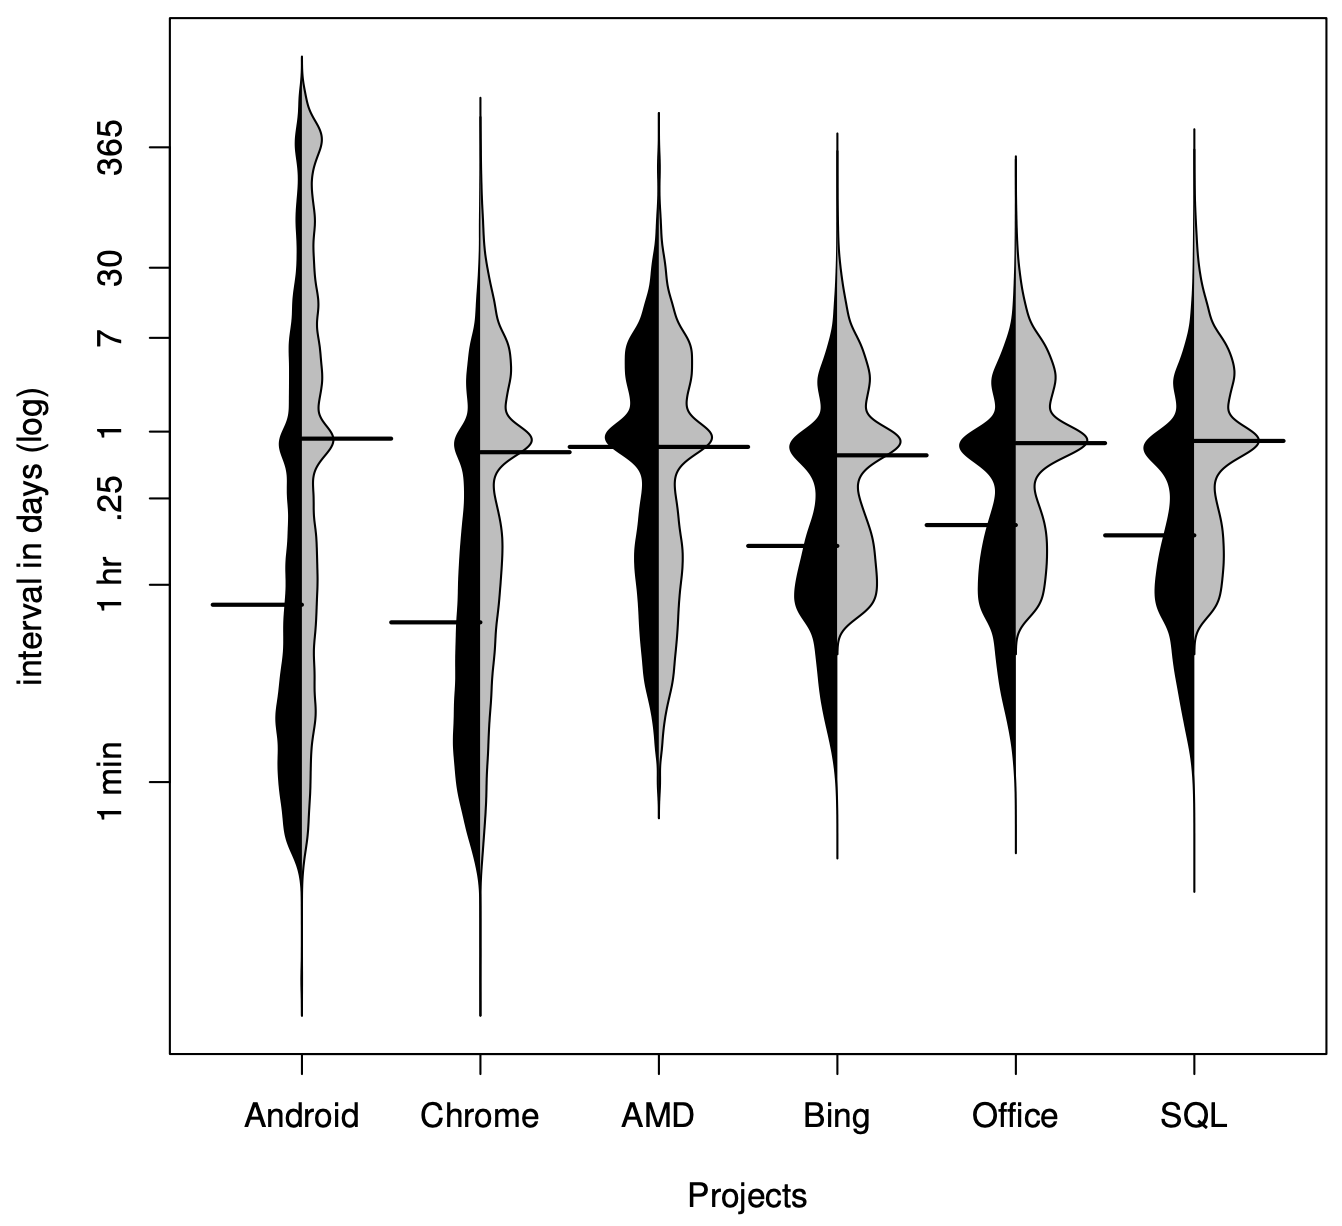
\includegraphics[width=.9\linewidth]{days-per-pr.png}
  \par\columnbreak\par
  ``AMD has short review intervals, with the median review taking \ul{17.5 hours}. Bing, SQL, and Office: \ul{14.7}, \ul{19.8}, and \ul{18.9 hours} respectively. The median completion time is \ul{15.7} and \ul{20.8 hours}, for Chrome and Android, respectively.''
  \source{rigby2013convergent}
  \end{multicols}}

\thought[bugayenko2015blog0622]{Reject it, if it lowers code coverage}

\pitch{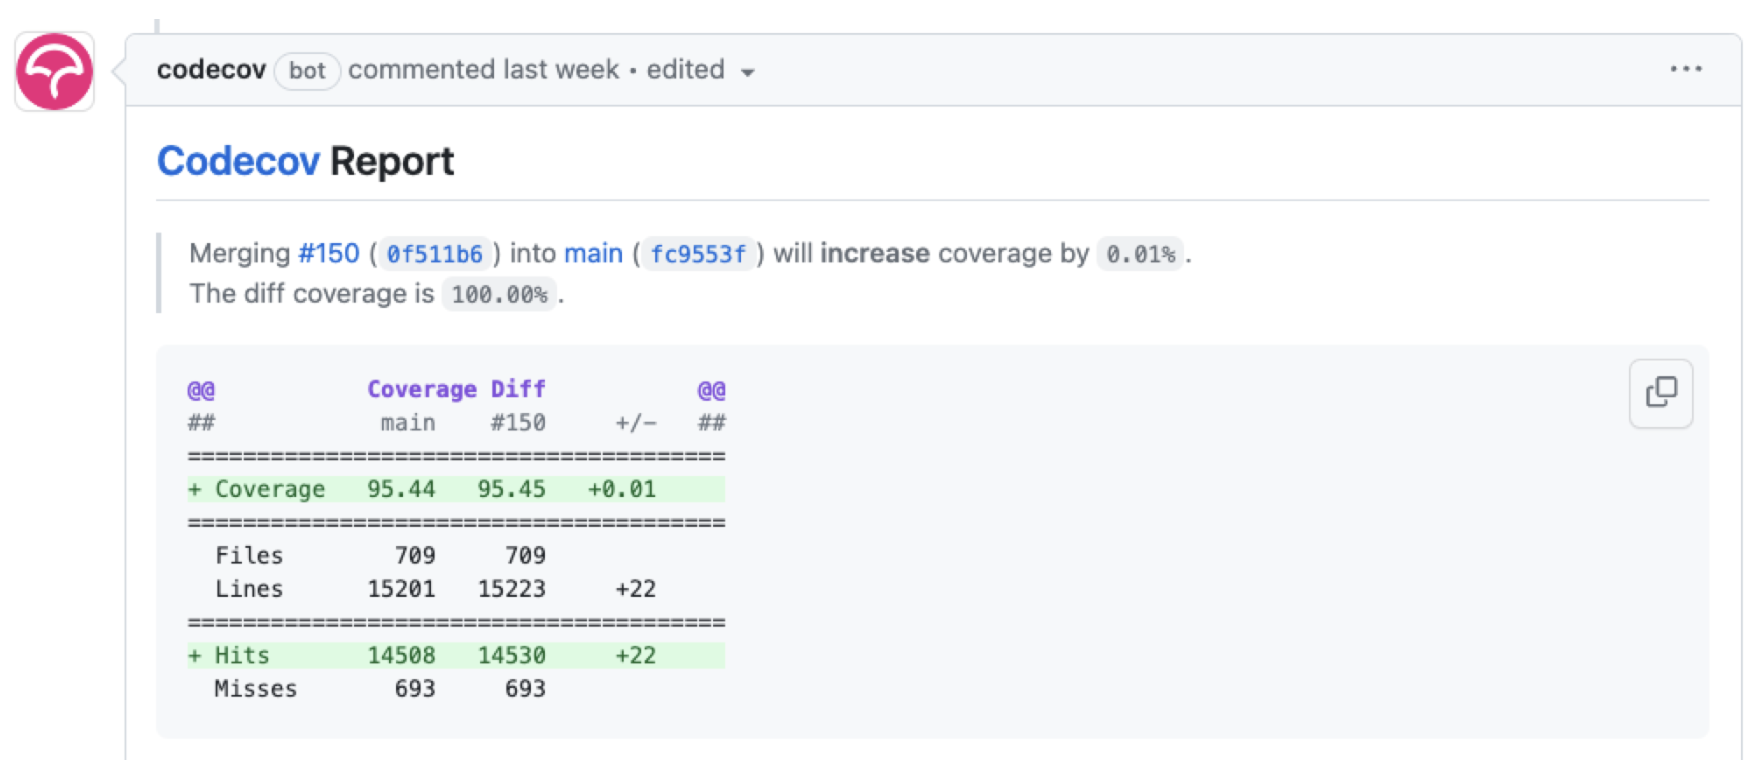
\includegraphics[width=.9\linewidth]{codecov.png}
\par{\small\url{https://docs.codecov.com/docs/pull-request-comments}\par}}

\thought[bugayenko2015blog0622]{Reject it, if it doesn't reproduce a bug}

\thought{Rely on the CI status, but not too much}

\qte
  [\nospell{\nospell{Mairieli Wessel}}]
  {mairieli-wessel}
  {Our findings also suggest that the adoption of GitHub Actions leads to \ul{more rejections} of pull requests (PRs), more communication in accepted PRs and less communication in rejected PRs, fewer commits in accepted PRs and more commits in rejected PRs, and \ul{more time} to accept a PR.}
  {wessel2023github}

\thought{Employ ChatGPT}

\pitch{
  \begin{multicols}{2}
  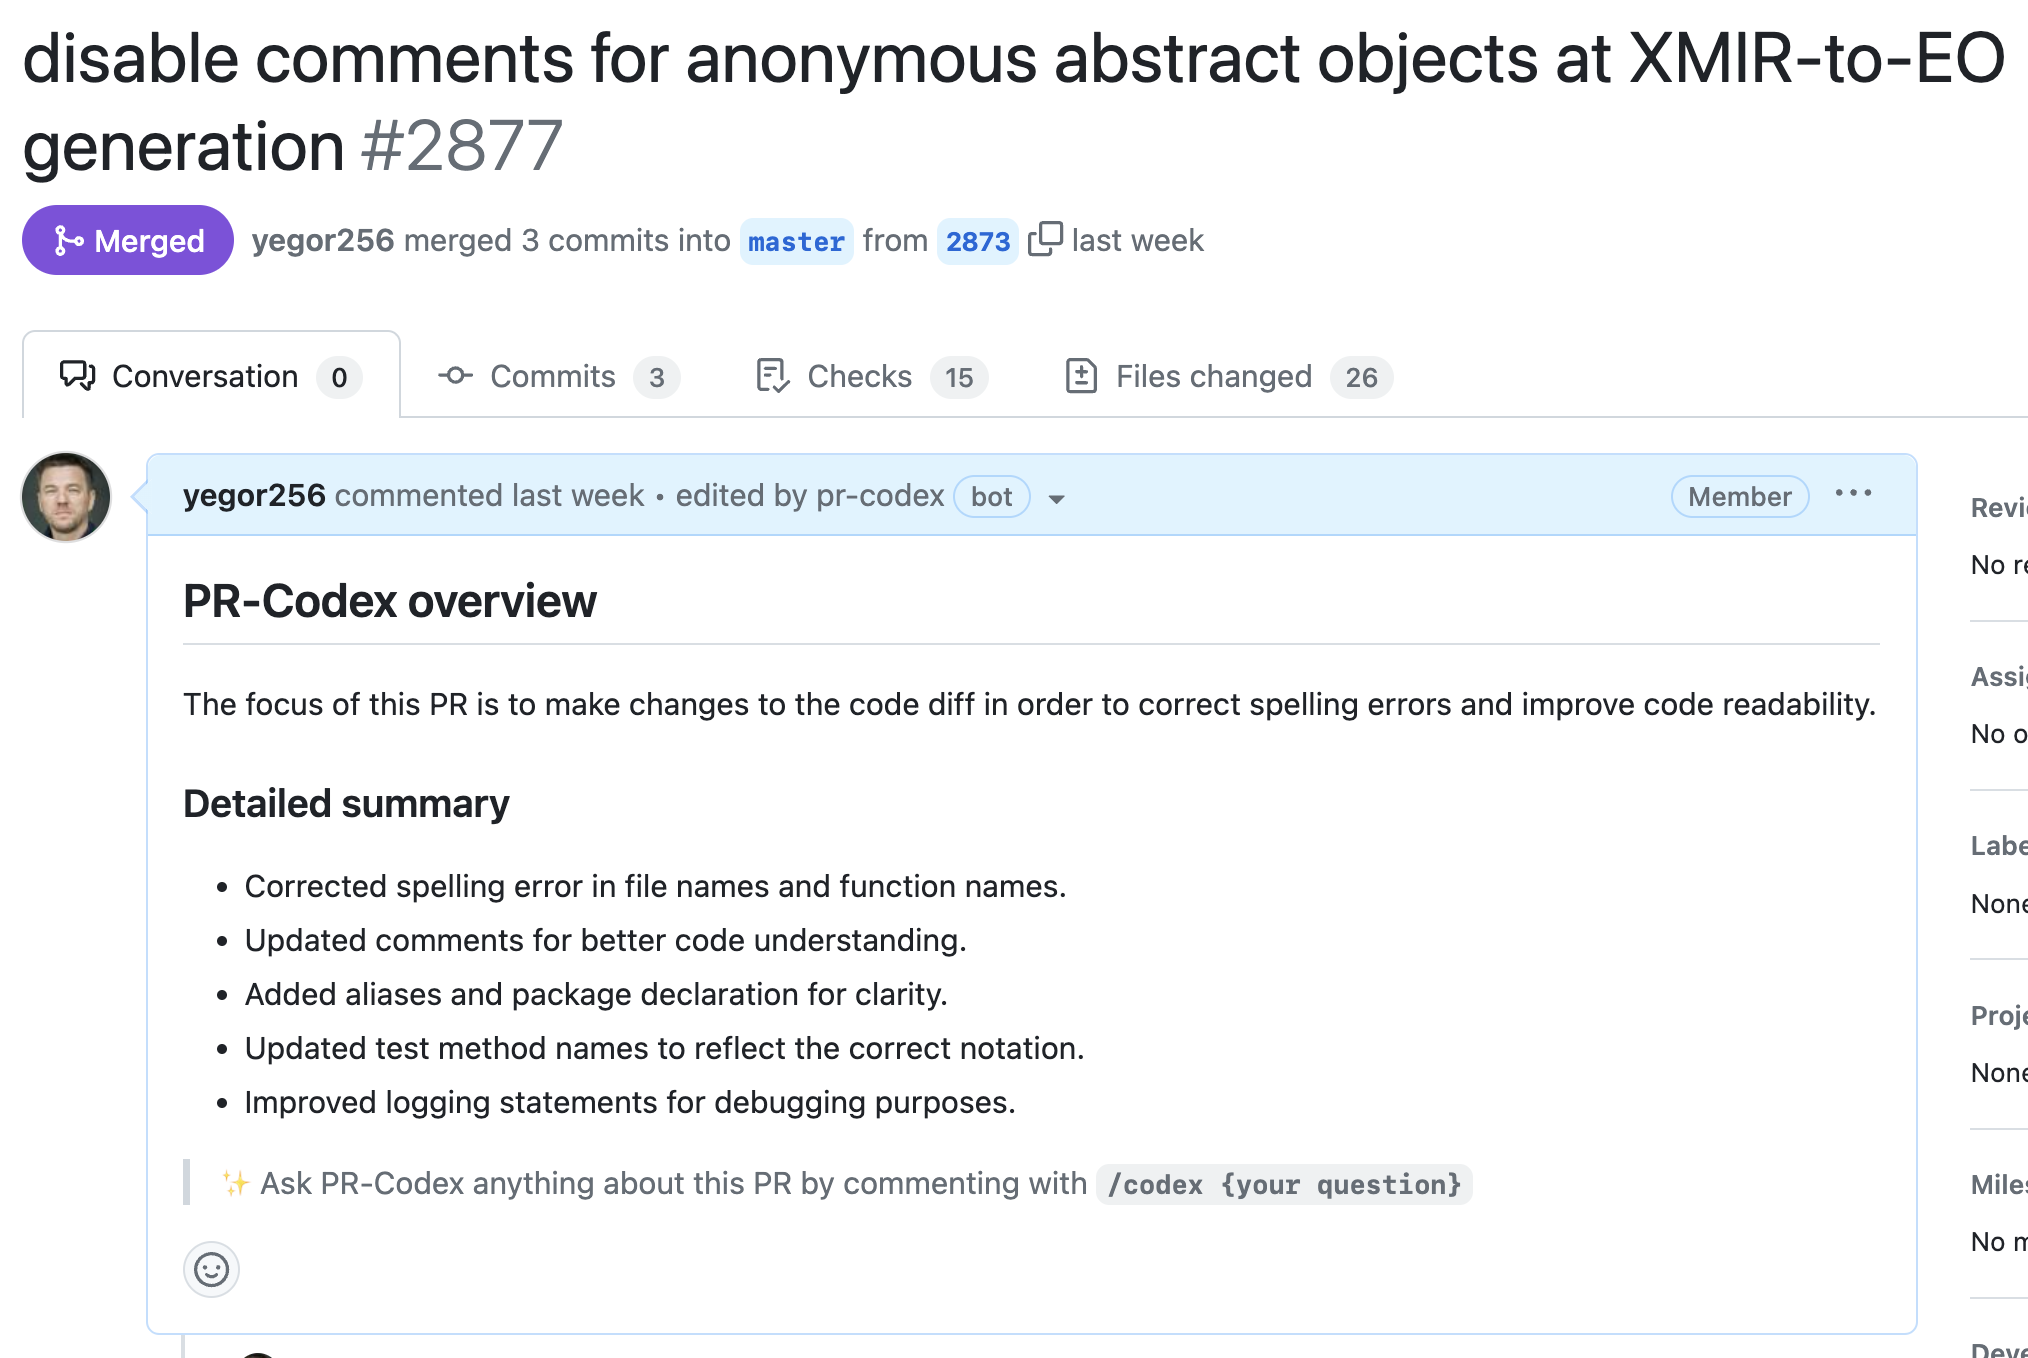
\includegraphics[width=.9\linewidth]{../03-making-changes/pr.png}
  \par\columnbreak\par
  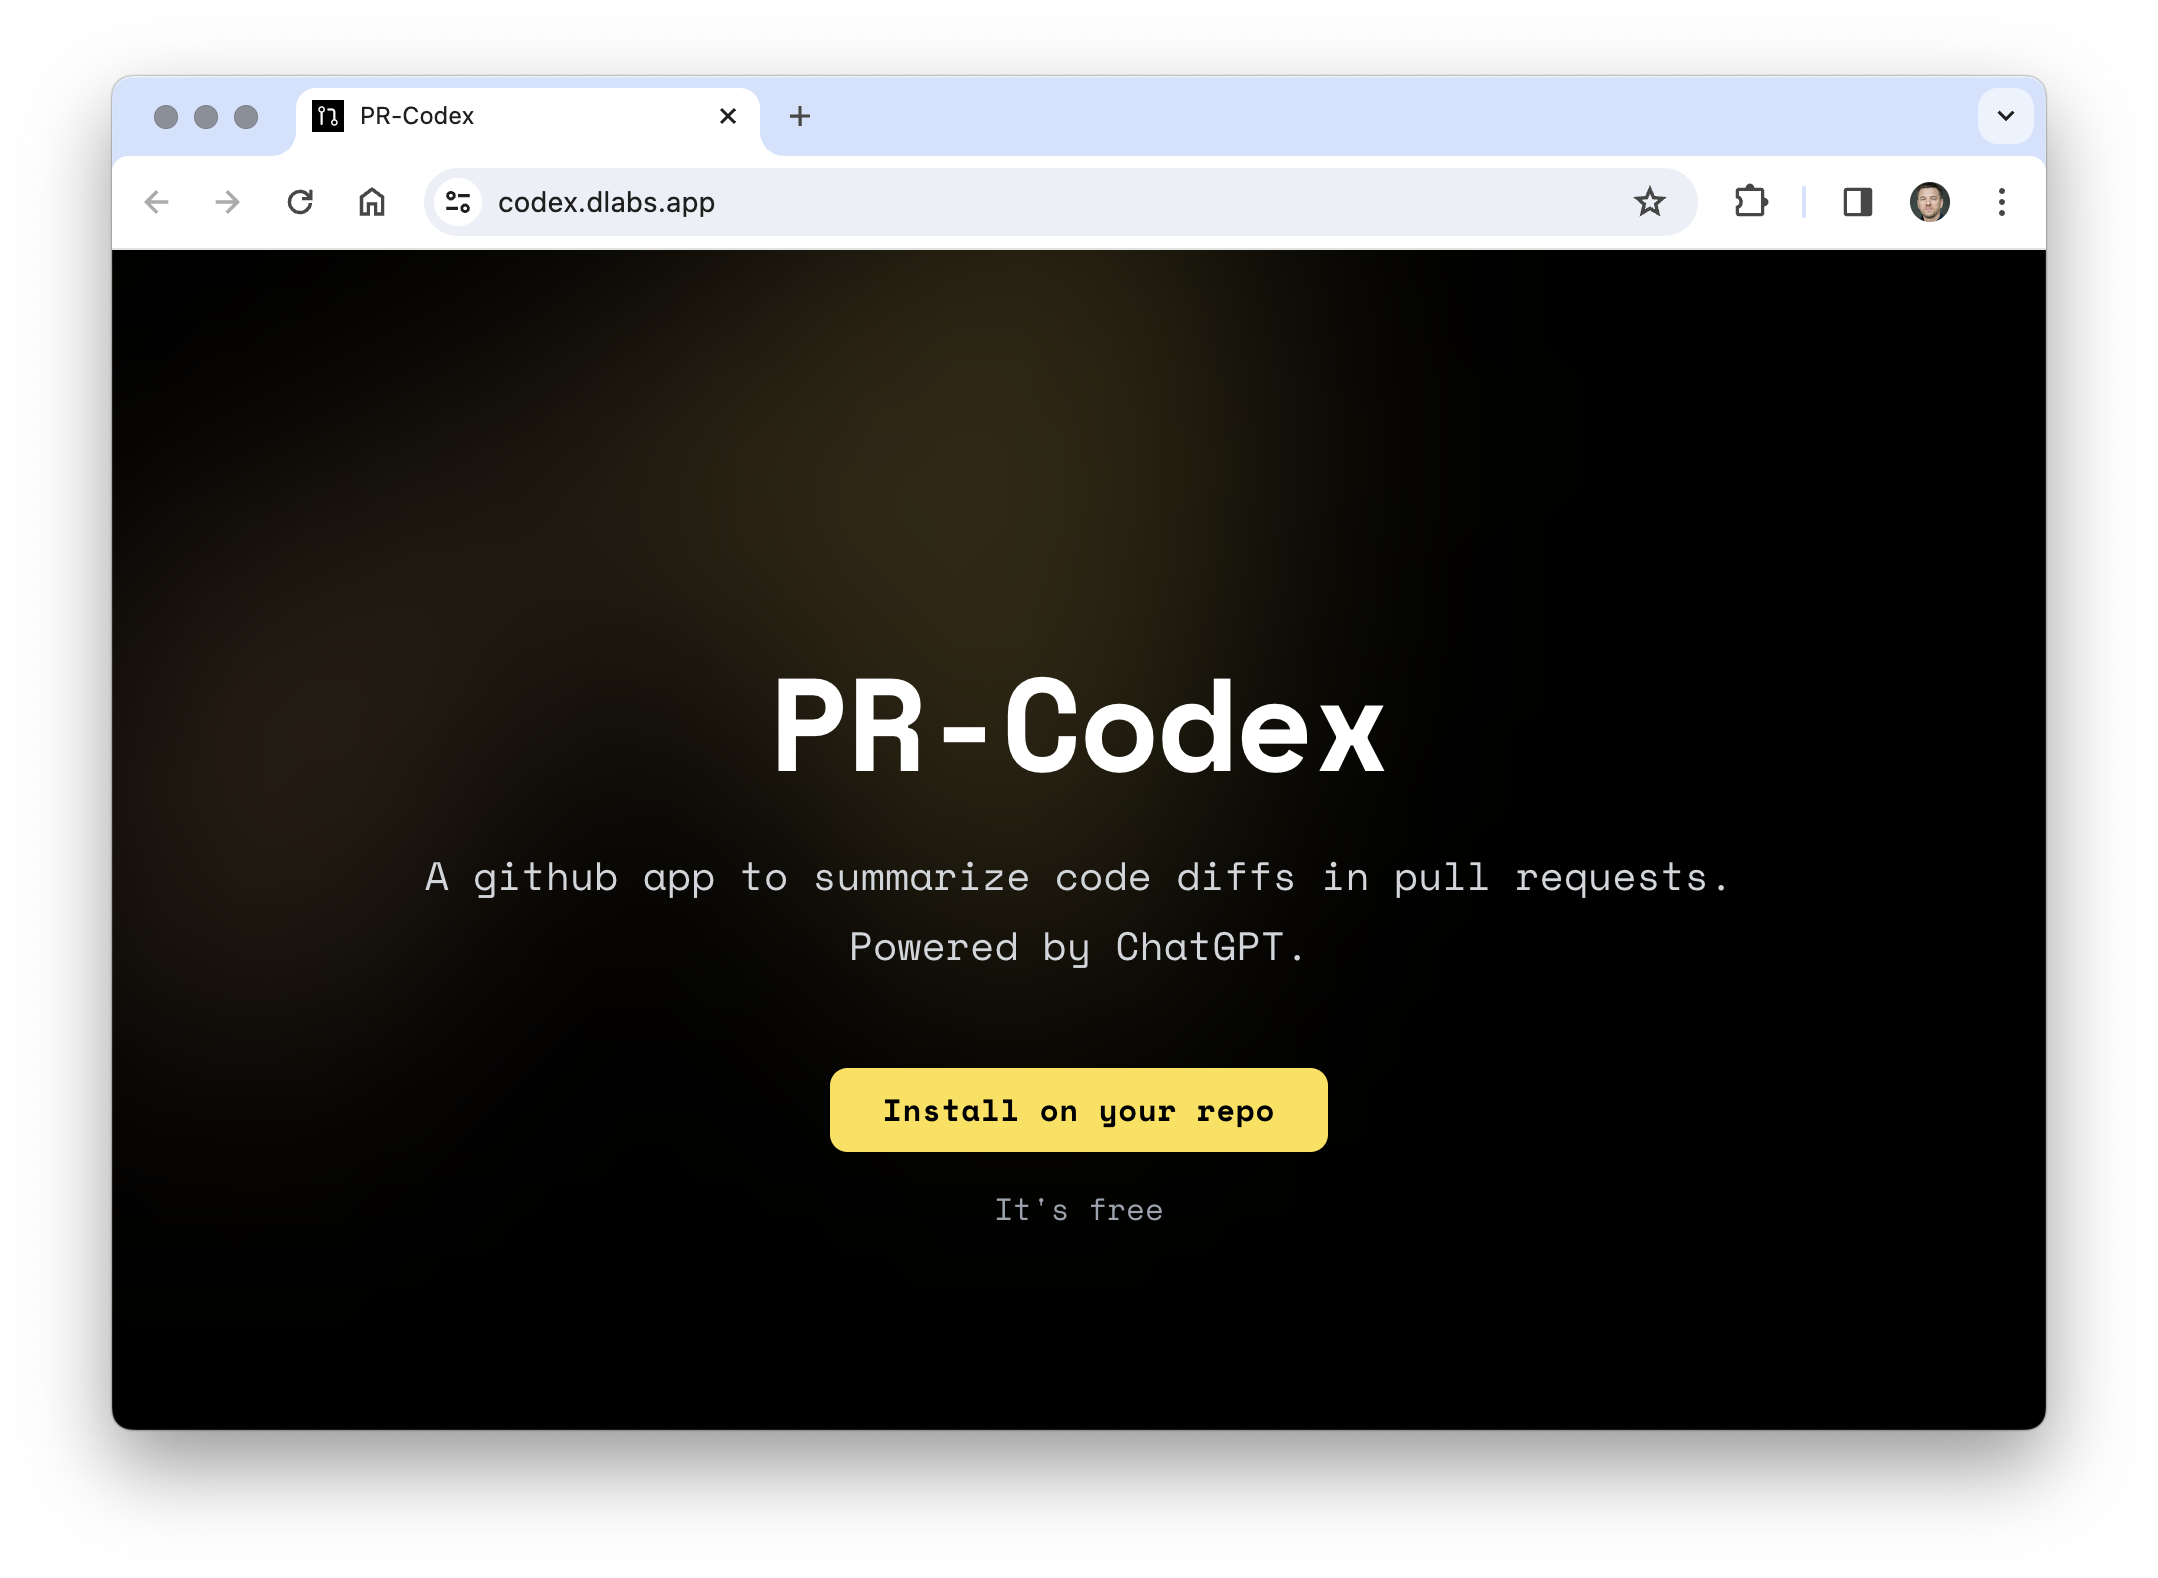
\includegraphics[width=.9\linewidth]{../03-making-changes/pr-codex.png}
  \end{multicols}
}

\end{document}
